\documentclass[12pt]{article}

% Packages
\usepackage[margin=1in]{geometry}   % Set page margins to 1 inch
\usepackage{fancyhdr}   % Allows customization of headers and footers
\usepackage{hyperref}   % Create hyperlinks in the document for easier navigation
\usepackage{datetime}   % For formatting the current date in various styles
\usepackage{parskip}    % Adds space between paragraphs and removes paragraph indents for better readability
\usepackage{amsmath}    % Provides advanced mathematical typesetting capabilities
\usepackage{amssymb}    % Provides additional mathematical symbols
\usepackage{multicol}   % Supports multi-column formatting in the document
\usepackage{graphicx}   % Allows inclusion and manipulation of graphics



% Hyperlink settings
\hypersetup{
    colorlinks=true, % Colored links instead of boxes
    urlcolor=blue,   % Blue color for external links
}

% Custom date format
\newdateformat{monthyeardate}{%
\monthname[\THEMONTH] \THEYEAR}

% Header settings
\pagestyle{fancy}
\fancyhf{}    % Clear all header and footer fields
\lhead{MATH 440 \\ 2:00 PM - 3:20 PM}         % Left header with class number and time
\rhead{Marty Martin \\ \monthyeardate\today}  % Right header with your name and the date
\renewcommand{\headrulewidth}{0.4pt}          % Header underlining
\setlength{\headheight}{54pt}                 % Ensure there's enough space for two lines in the header

\begin{document}

\begin{center}
  \Large \textbf{Practice for the exam}
\end{center}

% Section for Question 1
\section*{Question 1}
Suppose the random variables \(X\) and \(Y\) are jointly distributed according to the pdf:
\[ f_{XY}(x,y) = 8xy, \quad 0 < y < x < 1 \]
\begin{itemize}
  \item[(a)] Find \( P(X < 2Y) \)
  \item[(b)] Find \( P(Y < \frac{1}{4} |  x = \frac{1}{2}) \)
\end{itemize}


% Process for Question 1
\section*{Process}
% Legend for Question 1
\begin{itemize}
  \item \( X \): Random variable representing the first dimension
  \item \( Y \): Random variable representing the second dimension
  \item \( f_{XY}(x, y) \): Joint probability density function of \( X \) and \( Y \)
  \item \( f_X(x) \): Marginal probability density function of \( X \)
  \item \( f_{Y|X}(y|x) \): Conditional probability density function of \( Y \) given \( X \)
  \item \( P(X < 2Y) \): Probability that \( X \) is less than \( 2Y \)
  \item \( P(Y < \frac{1}{4} | X = \frac{1}{2}) \): Conditional probability that \( Y \) is less than \( \frac{1}{4} \) given \( X = \frac{1}{2} \)
\end{itemize}
% Part (a) explanation and calculation
\subsubsection*{Part (a) Find \( P(X < 2Y) \)}
\textbf{General Formula:}
For any joint PDF \( f_{XY}(x, y) \), the probability \( P(g(X, Y)) \) for some condition \( g \) is given by:
\[ P(g(X, Y)) = \int \int_{g(x, y)} f_{XY}(x, y) \, dx \, dy \]

\textbf{Specific Calculation:}
This probability calculation involves integrating the joint PDF over the region defined by \( X < 2Y \) and within the given bounds of \( 0 < y < x < 1 \).
\[
  P(X < 2Y) = \int_0^1 \int_0^{X/2} 8xy \, dy \, dx
\]
This integral setup reflects the condition \( X < 2Y \) within the area bounded by \( 0 < y < x < 1 \).

\textbf{Integration Steps:}
Calculate the inner integral over \( y \):
\[
  \int_0^{X/2} 8xy \, dy = 8x \left[ \frac{y^2}{2} \right]_0^{X/2} = 8x \left[ \frac{(X/2)^2}{2} \right] = X^3
\]
Now integrate with respect to \( x \):
\[
  \int_0^1 X^3 \, dx = \left[ \frac{X^4}{4} \right]_0^1 = \frac{1}{4}
\]

Thus, \( P(X < 2Y) = \frac{1}{4} \).

% Part (b) explanation and calculation
\subsubsection*{Part (b) Find \( P(Y < \frac{1}{4} |  x = \frac{1}{2}) \)}
\textbf{General Formula:}
For any joint PDF \( f_{XY}(x, y) \), the conditional probability \( P(A | B) \) is given by:
\[ P(A | B) = \frac{\int \int_{A \cap B} f_{XY}(x, y) \, dx \, dy}{\int \int_B f_{XY}(x, y) \, dx \, dy} \]

\textbf{Specific Calculation:}
Given \( X = \frac{1}{2} \), we need to find the conditional probability \( P(Y < \frac{1}{4} | X = \frac{1}{2}) \). This involves determining the conditional PDF \( f_{Y|X}(y|x) \) and integrating it over the desired range of \( Y \).

\textbf{Determine the Marginal Density of \( X \), \( f_X(x) \):}
The marginal density \( f_X(x) \) is found by integrating out \( Y \) from the joint PDF:
\[ f_X(x) = \int_0^x 8xy \, dy = 8x \left[ \frac{y^2}{2} \right]_0^x = 4x^3 \]
At \( x = \frac{1}{2} \), the marginal density \( f_X\left(\frac{1}{2}\right) \) is:
\[ f_X\left(\frac{1}{2}\right) = 4 \left(\frac{1}{2}\right)^3 = \frac{1}{2} \]

\textbf{Calculate the Conditional PDF \( f_{Y|X}(y|x) \):}
The conditional PDF \( f_{Y|X}(y|\frac{1}{2}) \) is:
\[ f_{Y|X}(y|\frac{1}{2}) = \frac{8 \cdot \frac{1}{2} \cdot y}{\frac{1}{2}} = 8y \]

\textbf{Compute the Conditional Probability \( P(Y < \frac{1}{4} | X = \frac{1}{2}) \):}
\[ P(Y < \frac{1}{4} | X = \frac{1}{2}) = \int_0^{1/4} 8y \, dy \]
Calculate the integral:
\[ \int_0^{1/4} 8y \, dy = \left[ 4y^2 \right]_0^{1/4} = 4 \left(\frac{1}{16}\right) = \frac{1}{4} \]

\textbf{Conclusion:}
Therefore, \( P(Y < \frac{1}{4} | X = \frac{1}{2}) = \frac{1}{4} \).

\newpage
% Subsection for Question 2
\section*{Question 2}
A random variable \( X \) has the moment generating function \( M_X(t) = \left(\frac{2+e^t}{3}\right)^9 \). Find \( \text{Var}(X) \).

\section*{Process}
\begin{itemize}
  \item \( X \): Random variable
  \item \( M_X(t) \): Moment generating function of \( X \)
  \item \( E(X) \): Expected value (mean) of \( X \)
  \item \( E(X^2) \): Second moment of \( X \)
  \item \( \text{Var}(X) \): Variance of \( X \)
\end{itemize}
\textbf{General Formula:}
% General formula for finding moments from MGF:
The moment generating function (MGF) \( M_X(t) \) of a random variable \( X \) is defined as \( M_X(t) = E(e^{tX}) \). The \( n \)-th moment of \( X \) is given by the \( n \)-th derivative of \( M_X(t) \) evaluated at \( t = 0 \):
\[ E(X^n) = M_X^{(n)}(0) \]

% Finding the first moment (mean) \( \mu \):
First, find the first derivative of \( M_X(t) \):
\[ M_X(t) = \left(\frac{2+e^t}{3}\right)^9 \]
\[ M_X'(t) = 9 \left(\frac{2+e^t}{3}\right)^8 \cdot \frac{e^t}{3} \]

Evaluate the first derivative at \( t = 0 \):
\[ M_X'(0) = 9 \left(\frac{2+e^0}{3}\right)^8 \cdot \frac{e^0}{3} = 9 \left(\frac{3}{3}\right)^8 \cdot \frac{1}{3} = 9 \cdot 1 \cdot \frac{1}{3} = 3 \]

Thus, the mean \( \mu \) of \( X \) is:
\[ \mu = E(X) = M_X'(0) = 3 \]

% Finding the second moment \( E(X^2) \):
Next, find the second derivative of \( M_X(t) \):
\[ M_X''(t) = \frac{d}{dt} \left[ 9 \left(\frac{2+e^t}{3}\right)^8 \cdot \frac{e^t}{3} \right] \]
Using the product rule:
\[ M_X''(t) = 9 \left[ 8 \left(\frac{2+e^t}{3}\right)^7 \cdot \frac{e^t}{3} \cdot \frac{e^t}{3} + \left(\frac{2+e^t}{3}\right)^8 \cdot \frac{e^t}{3} \right] \]

Evaluate the second derivative at \( t = 0 \):
\[ M_X''(0) = 9 \left[ 8 \left(\frac{3}{3}\right)^7 \cdot \frac{1}{3} \cdot \frac{1}{3} + \left(\frac{3}{3}\right)^8 \cdot \frac{1}{3} \right] \]
\[ M_X''(0) = 9 \left[ 8 \cdot 1 \cdot \frac{1}{9} + 1 \cdot \frac{1}{3} \right] \]
\[ M_X''(0) = 9 \left[ \frac{8}{9} + \frac{1}{3} \right] \]
\[ M_X''(0) = 9 \left[ \frac{8}{9} + \frac{3}{9} \right] \]
\[ M_X''(0) = 9 \cdot \frac{11}{9} = 11 \]

Thus, the second moment \( E(X^2) \) is:
\[ E(X^2) = M_X''(0) = 11 \]

% Finding the variance \( \text{Var}(X) \):
The variance of \( X \) is given by:
\[ \text{Var}(X) = E(X^2) - (E(X))^2 \]
\[ \text{Var}(X) = 11 - 3^2 = 11 - 9 = 2 \]

Therefore, the variance of \( X \) is:
\[ \text{Var}(X) = 2 \]


\newpage
% Subsection for Question 3
\section*{Question 3}
The driver of a truck loaded with 900 boxes of books will be fined if the total weight of the boxes exceeds 36450 pounds. If the distribution of the weight of a box has a mean of 40 pounds and a variance of 36, find the approximate probability that the driver will be fined.

\section*{Process}
% Introduce the problem setup:
\begin{multicols}{2}
  \textbf{Givens:}
  \begin{itemize}
    \item \( n = 900 \)
    \item \( \mu = 40 \) pounds
    \item \( \sigma^2 = 36 \) pounds\(^2\)
    \item \( T = 36450 \) pounds
  \end{itemize}

  \columnbreak

  \textbf{Legend:}
  \begin{itemize}
    \item \( n \): Number of boxes
    \item \( \mu \): Mean weight of a single box
    \item \( \sigma^2 \): Variance of the weight of a single box
    \item \( T \): Total weight threshold for the fine
    \item \( W \): Total weight of the 900 boxes
  \end{itemize}

\end{multicols}

\textbf{Symbols to Find:}
\begin{itemize}
  \item \( E(W) \): Expected total weight
  \item \( \text{Var}(W) \): Variance of the total weight
  \item \( \sigma_W \): Standard deviation of the total weight
  \item \( P(W > 36450) \): Probability of exceeding the weight threshold
\end{itemize}

\subsubsection*{Step 1: Determine the Distribution of the Total Weight}
Let \( X_i \) be the weight of the \( i \)-th box. The total weight \( W \) is:
\[ W = \sum_{i=1}^{900} X_i \]

Since the weights \( X_i \) are independently and identically distributed, \( W \) follows a normal distribution by the Central Limit Theorem (CLT):
\[ W \sim N(n\mu, n\sigma^2) \]

Calculate the mean and variance of \( W \):
\[ E(W) = n\mu = 900 \times 40 = 36000 \]
\[ \text{Var}(W) = n\sigma^2 = 900 \times 36 = 32400 \]
\[ \sigma_W = \sqrt{32400} = 180 \]

% Step 2: Standardize the problem to find the probability using the standard normal distribution:
\subsubsection*{Step 2: Standardize the Problem}
We need to find \( P(W > 36450) \).

Convert this to the standard normal variable \( Z \):
\[ Z = \frac{W - E(W)}{\sigma_W} = \frac{W - 36000}{180} \]

Thus, we need to find:
\[ P\left( Z > \frac{36450 - 36000}{180} \right) = P(Z > 2.5) \]

% Step 3: Use the standard normal distribution table to find the probability:
\subsubsection*{Step 3: Find the Probability Using the Standard Normal Distribution Table}
From the standard normal distribution table, \( P(Z > 2.5) \) is the area to the right of \( Z = 2.5 \).

\[
  P(Z > 2.5) = 1 - P(Z \leq 2.5)
\]
From the Z-table, \( P(Z \leq 2.5) \approx 0.9938 \).

Therefore:
\[
  P(Z > 2.5) = 1 - 0.9938 = 0.0062
\]

Thus, the approximate probability that the driver will be fined is:
\[ P(W > 36450) \approx 0.0062 \]


\newpage
\section*{Question 4}
Suppose that the number of calls per hour to an answering service follows a Poisson distribution with rate \( \lambda = 4 \).
\begin{itemize}
  \item[(a)] What is the probability that fewer than 2 calls came in the first hour?
  \item[(b)] What is the probability that there will be no calls in the next two hours?
\end{itemize}

\section*{Process}

% Process for Part (a)
\subsection*{Part (a)} What is the probability that fewer than 2 calls came in the first hour?

\subsubsection*{Step 1: Define the Poisson Distribution}
The number of calls per hour follows a Poisson distribution with parameter \( \lambda = 4 \).
\begin{itemize}
  \item \( \lambda \): Rate parameter of the Poisson distribution
  \item \( X \): Number of calls in the first hour
  \item \( P(X = k) \): Probability of getting exactly \( k \) calls in a given time period
  \item \( P(X < k) \): Probability of getting fewer than \( k \) calls in a given time period
\end{itemize}

\subsubsection*{Step 2: Probability Mass Function}
\textbf{General Formula:} The probability mass function of a Poisson random variable \( X \) with parameter \( \lambda \) is given by:

\[ P(X = k) = \frac{\lambda^k e^{-\lambda}}{k!} \]

\subsubsection*{Step 3: Calculate the Probability}
We need to find the probability that fewer than 2 calls came in the first hour, i.e., \( P(X < 2) \).

This can be calculated as:
\[ P(X < 2) = P(X = 0) + P(X = 1) \]

Using the Poisson pmf:
\[ P(X = 0) = \frac{4^0 e^{-4}}{0!} = e^{-4} \]
\[ P(X = 1) = \frac{4^1 e^{-4}}{1!} = 4e^{-4} \]

\subsubsection*{Step 4: Sum the Probabilities}
Therefore:
\[ P(X < 2) = e^{-4} + 4e^{-4} = 5e^{-4} \]

\subsubsection*{Step 5: Numerical Value}
Calculating the numerical value:
\[ P(X < 2) \approx 5 \times 0.0183 = 0.0915 \]

% Process for Part (b)
\subsection*{Part (b)} What is the probability that there will be no calls in the next two hours?

\subsubsection*{Step 1: Define the Poisson Distribution for Two Hours}
The number of calls in two hours also follows a Poisson distribution, but with parameter \( \lambda = 2 \times 4 = 8 \).
\begin{itemize}
  \item \( \lambda \): Rate parameter of the Poisson distribution
  \item \( Y \): Number of calls in the next two hours
  \item \( P(Y = k) \): Probability of getting exactly \( k \) calls in a given time period
  \item \( P(Y < k) \): Probability of getting fewer than \( k \) calls in a given time period
\end{itemize}

\subsubsection*{Step 2: Probability Mass Function}
We need to find the probability of no calls in the next two hours, i.e., \( P(Y = 0) \), where \( Y \sim \text{Poisson}(\lambda = 8) \).

\subsubsection*{Step 3: Calculate the Probability}
Using the Poisson pmf:
\[ P(Y = 0) = \frac{8^0 e^{-8}}{0!} = e^{-8} \]

\subsubsection*{Step 4: Numerical Value}
Calculating the numerical value:
\[ P(Y = 0) \approx 0.00034 \]


\newpage
\section*{Question 5}
Using moment generating functions (MGFs), show that if:
\[ X \sim N(\mu_1, \sigma_1^2) \quad \text{and} \quad Y \sim N(\mu_2, \sigma_2^2), \]
then the expectation and variance of \( X+Y \) are given by:
\[ E(X+Y) = \mu_1 + \mu_2 \quad \text{and} \quad \text{Var}(X+Y) = \sigma_1^2 + \sigma_2^2, \]
and that:
\[ X + Y \sim N(\mu_1 + \mu_2, \sigma_1^2 + \sigma_2^2). \]
\textit{Note:} The moment generating function of \( X \), if \( X \) is normally distributed, is given by:
\[ M_X(t) = e^{t\mu + \frac{t^2\sigma^2}{2}}. \]

\section*{Process}
\begin{itemize}
  \item \( \mu_1 \): Mean of the normal distribution for \( X \)
  \item \( \sigma_1^2 \): Variance of the normal distribution for \( X \)
  \item \( \mu_2 \): Mean of the normal distribution for \( Y \)
  \item \( \sigma_2^2 \): Variance of the normal distribution for \( Y \)
  \item \( M_X(t) \): Moment generating function of \( X \)
  \item \( M_Y(t) \): Moment generating function of \( Y \)
  \item \( M_{X+Y}(t) \): Moment generating function of \( X + Y \)
  \item \( E(X+Y) \): Expected value of \( X + Y \)
  \item \( \text{Var}(X+Y) \): Variance of \( X + Y \)
\end{itemize}
\subsection*{Step 1: Moment Generating Function (MGF) of a Normal Distribution}
The moment generating function (MGF) of a normally distributed random variable \( X \sim N(\mu, \sigma^2) \) is given by:
\[ M_X(t) = e^{t\mu + \frac{t^2\sigma^2}{2}} \]

\subsection*{Step 2: MGF of the Sum of Two Independent Normal Variables}
If \( X \sim N(\mu_1, \sigma_1^2) \) and \( Y \sim N(\mu_2, \sigma_2^2) \), the MGF of \( X + Y \) can be found using the property that the MGF of the sum of independent random variables is the product of their MGFs:
\[ M_{X+Y}(t) = M_X(t) \cdot M_Y(t) \]

Given:
\[ M_X(t) = e^{t\mu_1 + \frac{t^2\sigma_1^2}{2}} \]
\[ M_Y(t) = e^{t\mu_2 + \frac{t^2\sigma_2^2}{2}} \]

The MGF of \( X + Y \) is:
\[ M_{X+Y}(t) = e^{t\mu_1 + \frac{t^2\sigma_1^2}{2}} \cdot e^{t\mu_2 + \frac{t^2\sigma_2^2}{2}} \]

Using properties of exponents:
\[ M_{X+Y}(t) = e^{t\mu_1 + \frac{t^2\sigma_1^2}{2} + t\mu_2 + \frac{t^2\sigma_2^2}{2}} \]
\[ M_{X+Y}(t) = e^{t(\mu_1 + \mu_2) + \frac{t^2(\sigma_1^2 + \sigma_2^2)}{2}} \]

\subsection*{Step 3: Identifying the Distribution}
The MGF of \( X + Y \):
\[ M_{X+Y}(t) = e^{t(\mu_1 + \mu_2) + \frac{t^2(\sigma_1^2 + \sigma_2^2)}{2}} \]

This is the MGF of a normal distribution with mean \( \mu_1 + \mu_2 \) and variance \( \sigma_1^2 + \sigma_2^2 \). Therefore:
\[ X + Y \sim N(\mu_1 + \mu_2, \sigma_1^2 + \sigma_2^2) \]

\subsection*{Step 4: Expectation and Variance of \( X + Y \)}
\subsubsection*{Expectation}
The expectation of \( X + Y \) is:
\[ E(X + Y) = \mu_1 + \mu_2 \]

\subsubsection*{Variance}
The variance of \( X + Y \) is:
\[ \text{Var}(X + Y) = \sigma_1^2 + \sigma_2^2 \]

\section*{Conclusion}
We have shown that if \( X \sim N(\mu_1, \sigma_1^2) \) and \( Y \sim N(\mu_2, \sigma_2^2) \), then:
\[ E(X + Y) = \mu_1 + \mu_2 \]
\[ \text{Var}(X + Y) = \sigma_1^2 + \sigma_2^2 \]
\[ X + Y \sim N(\mu_1 + \mu_2, \sigma_1^2 + \sigma_2^2) \]

\begin{figure}[ht]
  \centering
  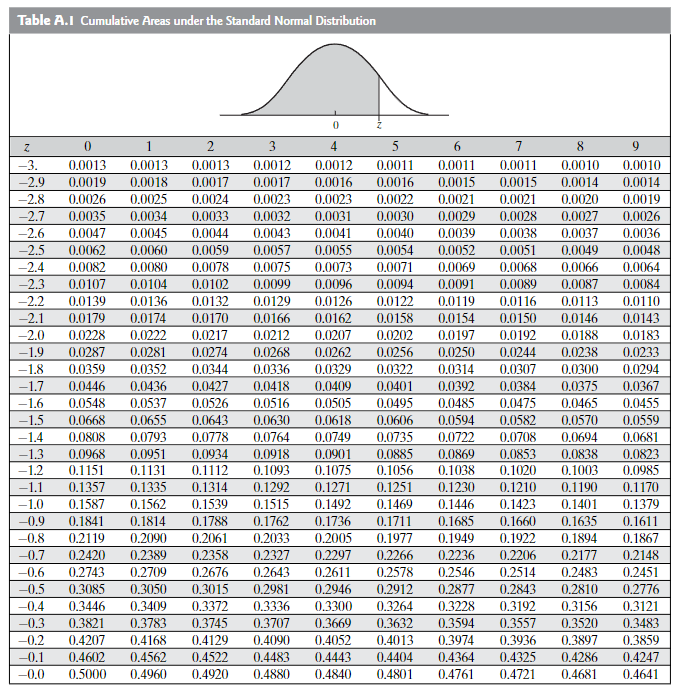
\includegraphics[width=\textwidth]{images/z-table_1.png}
  \caption{Cumulative Areas under the Standard Normal Distribution (Part 1)}
\end{figure}

\begin{figure}[ht]
  \centering
  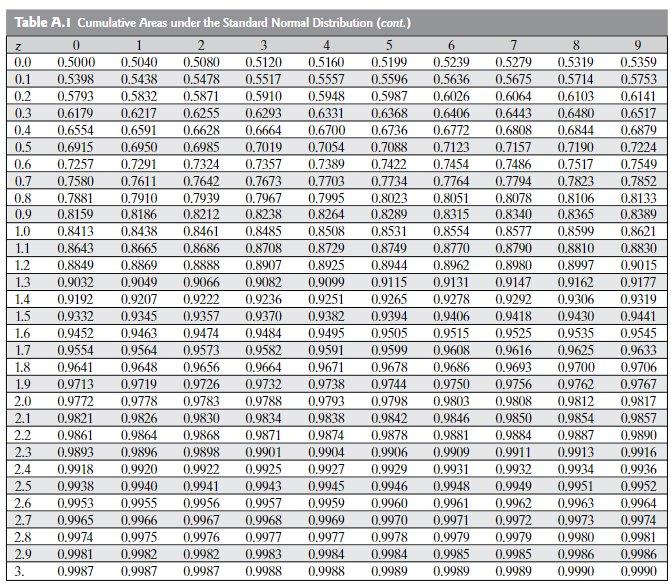
\includegraphics[width=\textwidth]{images/z-table_2.png}
  \caption{Cumulative Areas under the Standard Normal Distribution (Part 2)}
\end{figure}


\end{document}
